\documentclass[10pt,a4paper, twocolumn]{article}
\usepackage[utf8]{inputenc}
\usepackage[english]{babel}
\usepackage{amsmath}
\usepackage{amsfonts}
\usepackage{amssymb}
\usepackage{graphicx}
\usepackage{hyperref}
\usepackage{booktabs}
\usepackage{tablefootnote}
\usepackage[style=ieee]{biblatex}

\author{Diego Ballesteros, Trajche Kralev, Tribhuvanesh Orekondy}
\title{DJ Byg Data \\ \hspace{10pt} \\ \small{A project for the ETH Big Data course}}
\date{\today}
\addbibresource[datatype=bibtex]{report-3.bib}
\begin{document}
  \maketitle
  
  \begin{abstract}
  	DJ Byg Data was born out of curiosity about the data presented in
  	\cite{RapperWords}, it led to the question \textit{Can we say something about songs
  	based solely on their lyrics?}.
  	
  	The solution developed in this project focuses on genre
  	as the classifying trait for tracks and utilized unsupervised learning, namely
  	clustering, to discern tracks from each other; this reduced the dataset
  	from hundreds of thousands of points to 10 or 20 classes, which made it possible for
  	a human to define which genres are defined by each cluster. 
  	
  	The clustering implementation in a distributed computing environment,
  	specifically using Apache Spark
  	\footnote{https://spark.apache.org/} and Hadoop's MapReduce
  	\footnote{http://hadoop.apache.org/}, allowed the processing of about 280,000
  	tracks. The results of this implementation showed
  	that it is possible to identify the genre for clusters of songs based only
  	in features derived from their lyrics. Although in most cases the use of different
  	languages is the defining trait, the solution could still provide insight about
  	genres in English songs.
  \end{abstract}

  \section{Introduction}
	The research field of Music Information Retrieval (MIR) has been active for quite some
	time \cite{nameThatTune:1993} and its applications can be seen in several commercial
	products such as Pandora or Spotify \cite{recommendation:2010}. The development of
	large scale MIR systems is of interest not only to the research community, but
	potentially to the general public, however there is a number of challenges
	to address and one of them is the representational challenge
	and the choice of features to use when analyzing the musical data
	\cite{ARIS:ARIS1440370108}. 
	
	Currently a large number of research in the field is
	dedicated to song meta-data and audio features \cite{McFee:2012:MSD:2187980.2188222},
	however in this project the focus is set only on textual content, namely lyrics, as
	the main feature of the data. This choice is motivated by the intuition that
	songs can be treated similarly to documents in the traditional sense of
	Information Retrieval when they are reduced to its lyrical content, and using this
	approach opens up a wide range of possibilities given the existing research
	in document classification and analysis.
	
	As reported in \cite{doi:10.1300/J116v02n03_01}, identification based
	solely on lyrics may not be achievable. Nevertheless the solution developed
	in this project provides insights on how to enhance the current traditional
	solutions with lyric content and shows the potential of this approach.

  \section{Related work}

	The problem of identifying music genres is particularly challenging, even
	humans have problem at it because in many occasions the definition of a genre
	is not definitive and many songs sit in the boundary between multiple genres
	\cite{Li:2003:CSC:860435.860487}. There exists little research on
	feature extraction aiming towards genre classification, however
	usual approaches focus on audio features and supervised learning
	techniques \cite{1021072}.
	As mentioned in \cite{mckay2006musical}, these techniques
	are not very scalable to the volume of data available in the field. By following
	an unsupervised approach and a distributed computing paradigm, this projects
	aim to contribute to the problem of scalability in addition to the contribution
	to the use of lyrics as a feature for MIR.
	There is no direct quantitative comparison between the proposed approach and those
	present in the literature, however the final results suggest that this method
	is effective in real datasets and the use of lyrics feature in supervised settings
	could be explored and its quality assessed and compared with the state of the
	art methods.

  \section{Data model}
    \subsection{Introduction}

    One of the main limitations encountered during the small scale implementation
    we encountered during the first iteration of the project is that the
    intersection of the songs that have lyrics available in the musiXmatch
    dataset and at least one valid genre within the Last.fm tags is too small to
    produce significant results, in the small scale out of the $10000$ subset only
    $1400$ were left after filtering them with this criteria.
    
    In order to overcome this limitation, it was decided that for the scalable
    implementation, these tags would be ignored as a criteria for filtering or
    deciding a cluster's genre and instead they would be used only for quality
    metrics. This allowed the use of the full set of songs with lyrics in the
    million song dataset, the number of songs in this set is $237662$, i.e. 
    $23.7\%$ of the million song dataset.
    
    \subsection{Models}
    \subsubsection{Genre discovery}
    
    From the experience of the proof of concept, it was concluded that the
    clustering approach is adequate for the task at hand. And it is expected
    that with a larger amount of data it will be possible to distinguish
    more clearly the clusters and their genre correspondence. Therefore
    for the scalable implementation the clusters will be kept as the information
    model produced from the data.
    
    This allows for great scalability, because these clusters can be computed
    with a single pass on the data, in addition to the passes done to tune
    the parameters of the computation. Moreover, clusters allow for efficient
    updates if is to be received, since the usual K-means algorithms can
    be formulated in a streaming fashion.
    
    Additionally, it is also necessary to keep term frequencies and
    document frequencies in order to allow query points to be assigned
    to clusters and also the updated of these clusters with new data.
    
    \subsubsection{SQL database}
    In this project there exists a fortunate exception to the usual Big Data
    scenarios, the data has been cleaned and structured for academic and
    research purposes beforehand. Therefore, in light the quality of the data,
    it was decided that the approach to be used for the storage of the data would
    be a SQL database, namely a PostgreSQL database deployed on Amazon's RDS
    service.
 
    This option was chosen because of the following reasons:
 
    \begin{itemize}
      \item It reduces the complexity during the query phase which is used to
            compute statistics and quality metrics
      \item It is compatible with the processing model which requires only a
            single pass on the data, and then storage of the result. There
            is no need for scalability for writes.
      \item It can be scaled for read operations, by spawning read copies
            according to the load. This is possible because of the assumption
            that there is not new data often.
    \end{itemize}        
 
    The schema for the data is presented in figure \ref{fig:data_schema}.
 
    \begin{figure*}
      \centering
      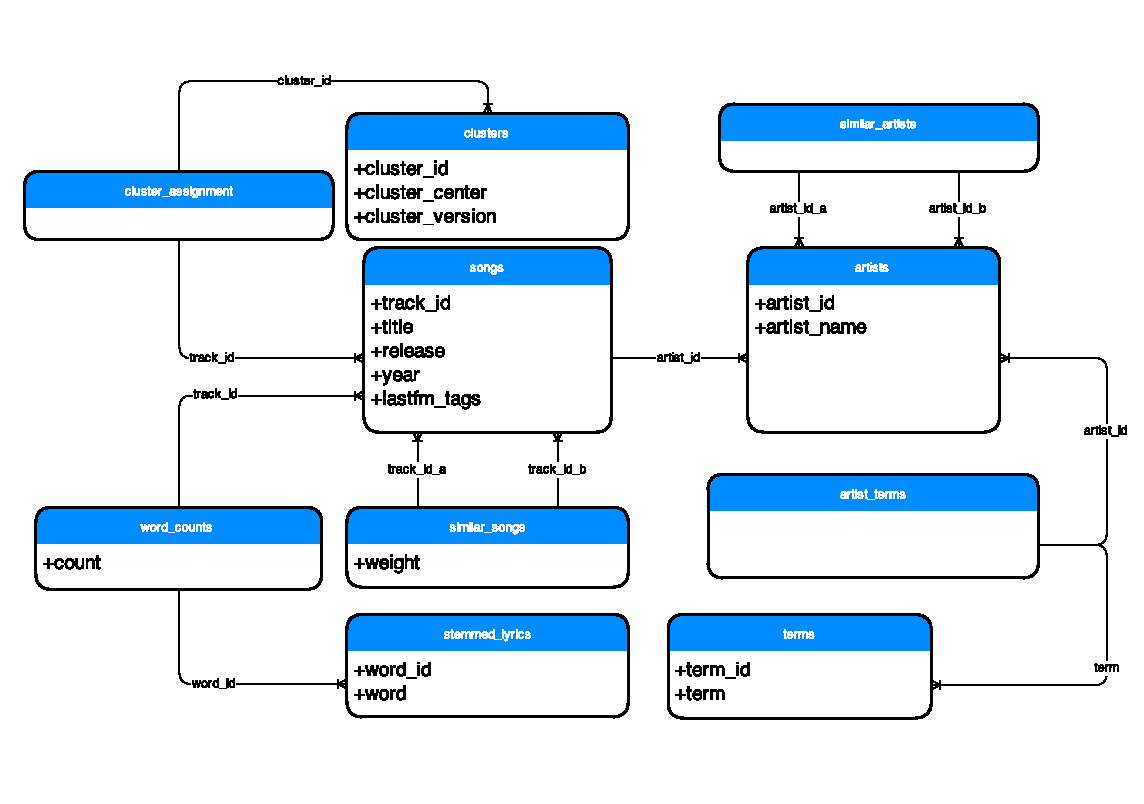
\includegraphics[scale=0.6]{img/database}
      \caption{SQL database schema}
      \label{fig:data_schema}
    \end{figure*}        

    \subsection{Preprocessing}
    \subsubsection{Lyrics preprocessing}
    \label{sec:preprocessing}

    For the processing of the data, i.e. clustering the songs based on their
    lyrics content, only the musiXmatch was required. This dataset is available
    as two zip files\footnote{These are provided as test and train dataset for
    academic purposes} where each file contains a single text file and in this
    file each line has the following format:
    
    \emph{track\_id,word\_id:count,word\_id:count,...}
    
    These files were merged and processed in a single machine to produce a file
    with a single 
    \emph{track\_id,word\_id,count} triplet per line. Additionally, the word id
    to stemmed word mapping was extracted from the header of the original files
    and stored in a separate file, it is important to note that this id is simply
    and index from 1 to 5000 which provides an ordering for the words.
    The resulting file with the word frequencies per track has 19M entries and a
    size of 450MB.
    
    The next step in the preprocessing of the lyrics was calculating the
    TF-IDF vectors for each song. Given the size of the input file and the
    natural parallelization of this task, it was decided to implement this
    step using MapReduce in a Hadoop cluster, namely in the AWS EMR service.
    To prepare for this computation, the input file was stored in an S3 bucket
    where it can be accessed by the cluster.
  
	  \subsection{Database preparation}
	
	  In order to fill up the SQL database with the rest of the information, it was
	  necessary to process the individual SQLite files provided with the dataset
	  and create CSV files that can be loaded quickly into the database tables.
	  The source files and the resulting database tables are summarized in table
	  \ref{tab:database_stats}.
	  
	  \begin{table*}
	    \centering
	    \caption{Database statistics}
	    \begin{tabular}{|c||c||c||c|}
	    \hline
	    Source & Source size & Target table & \# of records \\
	    \hline
	    track\_metadata.db & 685MB - 1M tracks & songs &
	    237662\tablefootnote{Only songs present in the musiXmatch dataset were
	    kept} \\
	    & & artists & 20521 \\
	    \hline
	    lastfm\_tags.db & 567MB - 8.5M (song, tag) pairs & songs &
	    173730\tablefootnote{This is the number of records with at least one tag}\\
	    \hline
	    artist\_term.db & 133MB - 1M (artist, term) pairs & terms & 6254\\
	    & & artist\_terms & 600570\\
	    \hline
	    lastfm\_similars.db & 3.8GB - 600k songs\tablefootnote{A single row
	    contains all the pairs associated with a song}
	    & similar\_songs & 8866734 \\
	    \hline
	    artist\_similarity.db & 322MB - 2M pairs & similar\_artists & 700608\\
	    \hline
	    \end{tabular}
	    \label{tab:database_stats}
	  \end{table*}     
  
  \section{System architecture}
  
  Figure \ref{fig:architecture} presents the different components of the system.
  
  \begin{figure*}
    \centering
    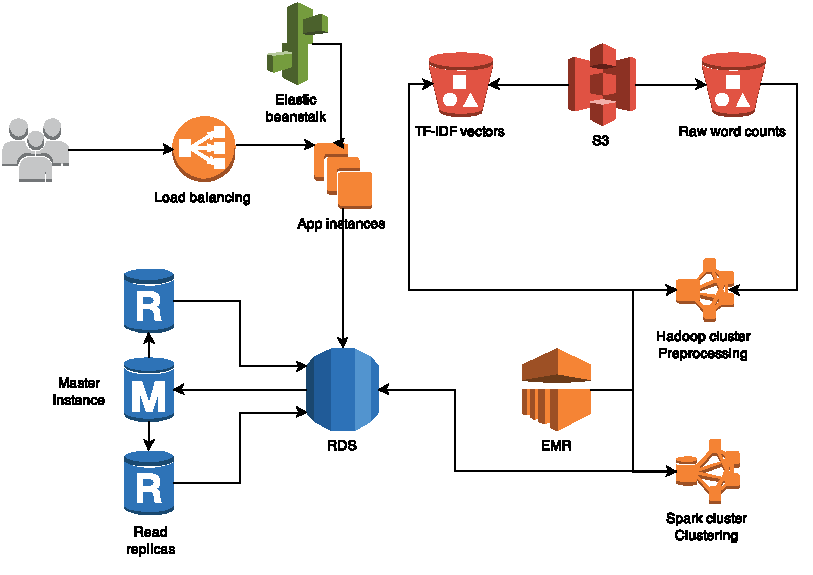
\includegraphics[scale=0.8]{img/architecture}
    \caption{System components}
    \label{fig:architecture}
  \end{figure*}          
      
  This system uses different services offered in AWS as building blocks for a
  scalable solution. In the following sections the different components will
  be introduced in more detail.
  
  \subsection{Preprocessing}

  The preprocessing component executes the workflow described in section
  \ref{sec:preprocessing}, the use of EMR and more specifically Hadoop's
  MapReduce provides great flexibility in regards on how big the input is, i.e.
  number of tracks and lyrics, because of the parallel nature of the
  calculation of TF-IDF vectors. Additionally, the use of S3 as a buffer for
  the data guarantees high performance as it is implemented using the Dynamo
  key-value store.
  
  \subsection{Storage}
  
  The RDS service provides also an scalable solution for read-heavy workloads
  as the ones for which the system is being designed, a single pass on the data
  produces the structured entities which are written only once into the system.
  Afterwards, what is expected of the system is to answer different queries from
  multiple users and in this case the use of read replicas allows horizontal
  scalability.
  
  \subsection{Compute}
 
  % What does the compute step do
  The compute step involves running the k-means algorithm for clustering.
  As input, it reads the TF-IDF vectors of all songs from S3.
  This in turn produces a list of cluster assignments and cluster centres which is 
  once again placed on to S3.
  
  % How it does it
  This step is implemented using Apache Spark's k-means$||$ algorithm.
  More specifically, it's a variant which uses an initialisation technique similar to k-means++,
  but which can executed in parallel.
  
  % Scaling benefits
  The performance benefits of running it on a Spark cluster was massive.
  The same code which took an hour to run on a local machine using 10\% of the dataset,
  took about 10 mins on a cluster with 8 large EC2 slave nodes for the complete dataset.
  This speed-up was for multiple reasons.
  For one, on a single machine, the data failed to fit in the memory.
  This was exacerbated by the fact that only 25\% of the dataset was cached in-memory and
  the remaining 75\% was read each time from S3, during each stage.
  We noticed reads of upto 500 MB in each stage.
  In contrast, when this was executed in a distributed environment, the data was partitioned on
  the worker nodes such that each worker node had access to a part of data locally.
  As a result, the entire dataset was cached in the cluster and we noticed reads of only
  6-7 MB per stage.
  
  \subsection{Interface}
  
  Finally, the system is exposed to the users via web interface which is deployed
  on AWS ElasticBeanstalk, this makes it possible to spin out EC2 instances on
  demand based on the load which guarantees the horizontal scalability of
  the system. Each of the application server instances holds no state, and simply
  executes the user queries against the database and renders the view, i.e.
  HTML/CSS/JS, with the results.
  
  With this architecture, it is possible to respond to an increasing number of
  users by either deploying a new EC2 instance or a read replica of the
  database. This has no hard limit on the computation side, and only
  would require considerations on the financial cost.
  
  \section{Experiments}
  Experiments were conducted using by varying two parameters - a) $k$, the number
  of clusters and b) $r$, the number of top-most occurring words in the lyrics.
  
  This section has been kept quite succinct due to the limited space available.
  We intend to explain each of the following results in much more detail in the next report.
  
  \subsection{Metrics}
  We evaluated our algorithm using four evaluation methods:
  \begin{enumerate}
  \item \textbf{Skewness of cluster sizes}. This measures how uniformly the songs are distributed among the clusters
  \item \textbf{Similar Songs}. The Last.fm dataset includes a list of similar songs pairs, and this is used to measure how such pairs were contained within a cluster.
  \item \textbf{Similar Artists}. Similar to the above metrics, except we take into account similar artist pairs.
  \item \textbf{Artists spread among clusters}, which measures how unique artists are for each cluster.
  \end{enumerate}
    
  \subsection{Results}
  We initially performed parameter exploration by setting $k$ to 5 to 20.
  This however did not yield good results, since the cluster sizes were extremely skewed.
  (In case of $k$ = 5, we noticed sizes of 198k, 39.5k, 2, 2 and 2.)
  This seemed to be a sign of using commonly occurring words into our feature vector.
  Hence, we proceeded to use another parameter $r$, which denotes the number of the most common words dropped from the feature vector.
  Using $r$ = 100, we obtained better results in terms of our metrics.
  
  The results obtained by using metrics 1, 2 and 4 are displayed in Tables \ref{tab:song_dis}, \ref{tab:res} and \ref{tab:num_artists_clusters} respectively.
  
\begin{table*}[h]
\centering
\caption{Distribution of songs among various clusters}
\begin{tabular}{@{}ll@{}}
\toprule
Cluster ID & \# Songs \\ \midrule
8           & 70770      \\
4           & 50898      \\
0           & 49324      \\
7           & 25387      \\
6           & 21078      \\
2           & 7545       \\
9           & 5967       \\
1           & 4993       \\
5           & 1697       \\
3           & 3          \\ \bottomrule
\end{tabular}
\label{tab:song_dis}
\end{table*}
  
\begin{table*}[h]
\centering
\caption{Similar song results obtained with $k = 5$ and $r = 100$}
\begin{tabular}{@{}llll@{}}
\toprule
Cluster ID & Recall             & Precision            & F1 score             \\ \midrule
0          & 0.317268888692571  & 0.00056390976856398  & 0.00112581852131951  \\
1          & 0.628220537658721  & 0.00423589820620664  & 0.00841505627160403  \\
2          & 0.0509420057673822 & 0.000558648814079117 & 0.00110517784055521  \\
3          & 0.0                   & 0.0                     &  0.0                    \\
4          & 0.369841836189631  & 0.000550576120332702 & 0.00109951541413113  \\
5          & 0.291016021091057  & 0.00598308891384352  & 0.0117251174894903   \\
6          & 0.829516889363635  & 0.00233533887959548  & 0.00465756531566462  \\
7          & 0.157993201293643  & 0.000498471326359098 & 0.000993807173622106 \\
8          & 0.438063048459549  & 0.000445161861024303 & 0.000889419889108439 \\
9          & 0.788758779343296  & 0.00726203303553385  & 0.0143915641992848   \\ \bottomrule
\end{tabular}
\label{tab:res}
\end{table*}

\begin{table*}[!t]
\caption{Uniqueness of artists to a cluster. For instance, this indicates that there exist 3 artists which appear in 8 clusters and 8228 artists that appear in only a single cluster}
\centering
\begin{tabular}{@{}ll@{}}
\toprule
\# Clusters & \# Artists \\ \midrule
1             & 8228         \\
2             & 3838         \\
4             & 3003         \\
3             & 2922         \\
5             & 2280         \\
6             & 218          \\
7             & 29           \\
8             & 3            \\ \bottomrule
\end{tabular}
\label{tab:num_artists_clusters}
\end{table*}
  
  \subsection{So, can it detect genres?}
  TODO: Expand with the items from point 5 from the last milestone
  Surprisingly, it does.
  We initially started off using the centroid of the clusters as being representative of the genres.
  However, this did not yield such meaningful results.
  One useful observation we did come across was that bad cluster centres, i.e, ones that have poor recall values, made use of extemely generic words.
  
  Cluster centroids need not however be representative of their songs.
  So, we proceeded to look at the artists and artist-tags contained in each cluster.
  This is where the pattern among clusters became clear.
  Few clusters were representative of the language of the lyrics, such as German, Spanish, French and Nordic.
  Furthermore, we also noticed clusters which were in English, and yet contained diverse genres.
  Examples include one containing death metal and another a combination of rap and rock.
  
  \printbibliography
\end{document}